\documentclass{./../../Latex/tests}
\begin{document}
\thispagestyle{plain}
\myheader{Sample Final Exam}
\rhead{Sample Final Exam}
\vspace{0.5em}
\testHeader{110}{40}

\newpage
%%%%%%%%%%%%%%%%%%%%%%%%%%%%%%%%%%%%%%%%% Question 1
\begin{enumerate}
\item (6 pts) Answer the following questions. (1 pt each)
\begin{enumerate}
\item What is the inverse of the function $f(x)= 4x + 6$? \\
\vspace{4cm}
\item  Find the intersection of the following sets:
$$ A = \{x: x>0 \} \quad \quad B = \{x: x\text{ is an even number} \} $$ 
\vspace{4cm}
\item  The inverse of a $4\times 4$ matrix $A$ exists if
\begin{itemize}
	\item[$\square$] The determinant of $A$ is 0 
	\item[$\square$] The determinant of $A$ is not 0 
	\item[$\square$] Rank of $A$ is 4
	\item[$\square$] Rank of $A$ is 0
	\item[$\square$] All rows of $A$ are linearly independent
\end{itemize}  
\textit{Select all that apply.}

\newpage
\item  Is the function $y=|x-1|$ differentiable at $x=1$? 
\begin{itemize}
	\item[$\square$] Yes. 
	\item[$\square$] No.
	\item[$\square$] Can't say. \\~\\
\end{itemize}  

% Part (e)
\item The function $f(K,L) = K^{\alpha} L^{1-\alpha}$ is:
\begin{itemize}
  \item[$\square$] Homogeneous of degree 0
  \item[$\square$] Homogeneous of degree 1
  \item[$\square$] Not homogeneous 
  \item[$\square$] Homogeneous but cannot say of what degree \\~\\
\end{itemize}

%\item What is the rank of the following matrix: $$A=\left[\begin{array}{rrr} 1 & 1 & 1 \\ 2 & 2 & 2 \\ 1 & 2 & 3\end{array}\right]$$

% Part (f)
\item The following function is:
\begin{center}
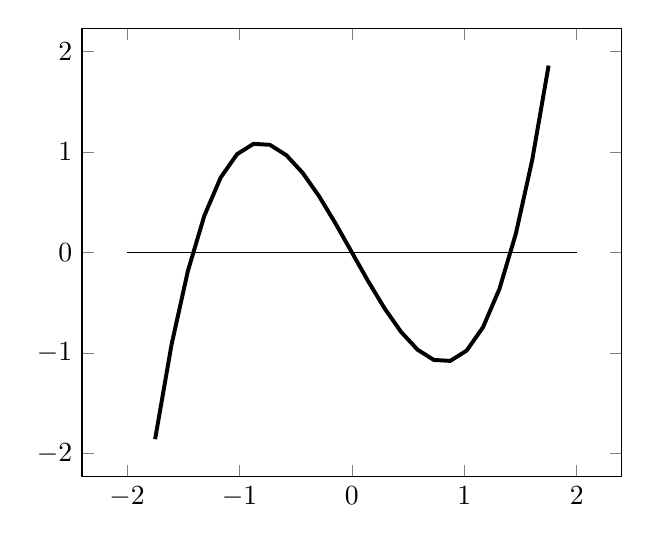
\begin{tikzpicture}
\begin{axis}[]
\addplot[color=black, line width=0.5mm, domain=-1.75:1.75] {x^3-2*x};
\addplot[domain=-2:2] {0};
\end{axis}
\end{tikzpicture} 
\end{center}
\begin{itemize}
  \item[$\square$] Quasiconcave
  \item[$\square$] Strictly quasiconcave
  \item[$\square$] Quasiconvex
  \item[$\square$] None of the above \\~\\
\end{itemize} 
\end{enumerate} 

\newpage

%%%%%%%%%%%%%%%%%%%%%%%%%%%%%%%%%%%%%%%%% Question 2
\item (5 pts) Consider a single-variable function:
 $$ y = f(x) $$
 In class, we learnt that at any local maximum or minimum, we must have that, 
 $$ f'(x^*) = 0 $$
 In addition, a sufficient condition for a critical point $x^*$ to be a local maximizer is:
 $$ f''(x^*) <0 $$ 
 \begin{enumerate}
  \item (2 pts) Why can't we have a maximum or minimum at a point where $f'(x)>0$ or $f'(x)<0$?
  \vspace{6cm} 
  \item (2 pts) Why is $f''(x) <0$ a sufficient condition for a critical point to be a maximizer?
  \vspace{6cm} 
  \item (1 pt) If $f$ is a strictly concave function, can we have two critical points, i.e., two distinct values of $x$ such that $f'(x_1) = f'(x_2) = 0$?
\end{enumerate}

\newpage
%%%%%%%%%%%%%%%%%%%%%%%%%%%%%%%%%%%%%%%%% Question 3
\item (5 pts) Prove the following statements:
\begin{enumerate}
\item (2 pts)  $ \sum_{i=1}^2 3 (x_i +1) = 3 \left(\sum_{i=1}^2 x_i \right)+ 6 $
\vspace{5cm}

\item (3 pts)  Given the following production function: 
$$ Q = f(K, L) = A K^{\alpha} L^{\beta} $$
The partial elasticity of output with respect to capital $K$ and labor $L$ is $\alpha$ and $\beta$, respectively. 


\end{enumerate} 

\vspace{1cm}

\newpage
%%%%%%%%%%%%%%%%%%%%%%%%%%%%%%%%%%%%%%%%% Question 4
\item (8 pts) \textit{Consider the following system of equations:
}\begin{align*}
x_1 + 2 x_2 = 6 \\
3 x_1 + x_2 = 3 \\
\end{align*}
\begin{enumerate}
\item (2 pts) \textit{Write this system of equations in matrix format i.e., $$ Av=b $$
What is $A$, $v$, and $b$ equal to?} 
\vspace{5.5cm}
\item (2 pts) \textit{Calculate the inverse of $A$. } 
\newpage \item (2 pts) \textit{If you premultiply $A^{-1}$ on both sides of the equation $ Av=b $, you should be able to derive an expression to solve for $v$. Write down this expression. } \\
\vspace{5.5cm}
\item (2 pts) \textit{Using the expression in $(c)$ solve for $v^*$. } 
\vspace{5cm}
\end{enumerate}

\newpage
%%%%%%%%%%%%%%%%%%%%%%%%%%%%%%%%%%%%%%%%% Question 5
\item (16 pts) You are given the following inter-temporal utility function:
$$ U = U(c_1, c_2) =  \ln c_1 + \beta \ln c_2 $$
where $c_1$ and $c_2$ is consumption in period 1 and 2, respectively. $0<\beta<1$ is the rate at which you discount the future and it measures your impatient. You earn income $y_1>0$ in period 1 and income $y_2>0$ in period 2. Any of the income you save $s$ in period 1 earns interest $r>0$. So, $$ c_1 + s = y_1, \quad \quad c_2 = y_2 + (1+r) s $$
Combining these constraints (plugging $s=y_1-c_1$ in the expression for $c_2$):
$$ c_1 + \frac{1}{1+r} c_2 = y_1 + \frac{1}{1+r} y_2 $$
Let the present-discounted income be denoted by $m$, such that:
$$ m = y_1 + \frac{1}{1+r} y_2 $$

\vspace{2em}
You want to choose $c_1$ and $c_2$ to maximize utility $$ U = U(c_1, c_2) =  \ln c_1 + \beta \ln c_2 $$ subject to the constraint:
$$ c_1 + \frac{1}{1+r} c_2 = m $$

\begin{enumerate}
	\item (2 pts) Write down the Lagrangian function corresponding to the above maximization problem. 
\newpage
	\item (3 pts) Write down the first-order conditions for a critical point. 
	\vspace{8cm}
	\item (3 pts) Using the first order conditions in (b), show that the optimal consumption $c_1^*$ and $c_2^*$ and the Lagrange multiplier $\lambda^*$ are given by:
	$$ c_1^* =\frac{m}{1+\beta}, \quad  c_2^* = \frac{\beta m(1+r)}{1+\beta}, \quad \lambda^* = \frac{1+\beta}{m} $$
	\vspace{8cm}
	
	\item (1 pt) Here, $U(c_1, c_2)$ is a strictly quasiconcave function. Is this sufficient to conclude that the $c_1^*$ and $c_2^*$ we found in (c) characterize a global maximum?
	\vspace{3cm}
	\item (2 pts) How does the optimal consumption in period 1 and 2 change due to an increase in $m$? Calculate $\partial c_1^*/\partial m$ and $\partial c_2^*/\partial m$ to answer your question. 
	\vspace{8cm}
	\item (1 pt) If $r=0$, using your expressions for $\partial c_1^*/\partial m$ and $\partial c_2^*/\partial m$, answer whether optimal consumption in period 1 changes by more or less than consumption in period 2 in response to a change in $m$?
	\newpage
	\item (2 pts) How does optimal consumption in period 1 change due to an increase in the interest rate $r$? \\
	
	Note that here, $$ m = y_1 + \frac{y_2}{1+r}  $$
	So to calculate $\partial c_1^*/\partial r$, you need to use the chain-rule as follows:
	$$ \frac{\partial c_1^*}{\partial r} = \frac{\partial c_1^*}{\partial m}\cdot \frac{\partial m}{\partial r}  $$
	\vspace{8cm}
	\item (2 pts) By how much does the maximum utility $U(c^*_1, c^*_2)$ change due to an increase in $m$? (Hint: What does $\lambda^*$ tell us?)
	\end{enumerate}

\end{enumerate}
\end{document}